\section{Analysis Procedure} \label{sec:ana}
% \begin{flushleft}
%    \subsection{Analysis overview}
The goal of TASEH is to find the axion signal hidden in the noise. In 
order to achieve this, the analysis procedure includes the following steps:
    \begin{enumerate}
        %\item Read raw data (I, Q) from tdms file and do Fast Fourier transform every 1 millisecond of spectrum, then average all over spectra in 1 second to get power spectrum.
        \item Perform fast Fourier transform (FFT) on the 
IQ time series data to obtain the frequency-domain power spectrum.
        \item Apply the Savitzky-Golay (SG) filter to remove the structure 
of the background in the frequency-domain power spectrum.
        \item Combine all the spectra from different frequency scans with 
the weighting algorithm.
        \item Merge bins in the combined spectrum to maximize the SNR. 
       \item Rescan the frequency regions with candidates and set limits on 
      the axion-two-photon coupling \gagg\ if no candidates were found.
    \end{enumerate}

    The analysis is done by following the procedure similar to that 
adopted by the HAYSTAC experiment ~\cite{HAYSTACII}.
% \end{flushleft}

%\subsection{Tdms}
\subsection{Fast Fourier transform}
\label{sec:FFT}
The in-phase $I(t)$ and quadrature $Q(t)$ components of the time-domain 
data were sampled and saved in the TDMS 
(Technical Data Management Streaming) files - a 
binary format developed by National Instruments.
%Fast Fourier Transform (FFT) was performed to convert the data into frequency-dependent and into unit of power by using the equation:
The FFT is performed to convert the data into 
frequency-domain power spectrum in which the measured power is calculated 
using the following equation:

\begin{equation}
\label{eq:4.1}
    \text{Power} = \frac{|\text{FFT}(I+i \cdot Q)|^{2}}{N \cdot 2R},
\end{equation}
where $N$ is the number of data points ($N  = 2000$ in the TASEH 
CD102 data), and $R$ is the input resistance of the signal analyzer 
(50~$\Omega$).
The FFT is done for every one-millisecond subspectrum data. The integration 
time for each frequency scan was about 32-42 minutes, which resulted 
in 1920000 to 2520000 subspectra; an average over these subspectra gives 
the averaged frequency-domain power spectrum for each scan. 
The frequency span in the spectrum from each resonant-frequency scan is 
1.6~MHz while the 
resolution is 1~kHz, giving 1600 frequency bins in each spectrum.  

%\subsection{Savitzky Golay filter}
\subsection{Remove the structure of the background}
%Figure \ref{fig:sg_result} is the spectrum in each step, somehow they all have a similar structure, in order to remove this structure, we will use a Savitzky Golay filter in every second to smooth the data Figure \ref{fig:After_Sg}.

In the absence of the axion signal, the output data spectrum is simply the 
noise from the cavity and the amplification chain. If axions are present 
in the cavity, the signal will be buried in the noise because the 
signal power is very weak. Therefore, the structure of the raw averaged 
output power spectrum, as shown in the upper panel of 
Fig.~\ref{fig:raw_sg_power}, is dominated 
by the noise of the system and an explanation for the structure can be found 
in Appendix~\ref{sec:cavitynoise}. The Savitzky Golay (SG) 
filter~\cite{SGFilter}, a digital filter that can smooth data without 
distorting the signal tendency, is applied to remove the structure of the  
background. The SG filter is performed on the averaged spectrum of each 
frequency scan by fitting adjacent points of successive sub-sets of data with 
an $n^\text{th}$-order polynomial. The result depends on two parameters: 
the number of 
data points used for fitting, the so-called window width, and the order of 
the polynomial. If the window is too wide, the filter will not remove small 
structures, and if it is too narrow, it may kill the signal. 
%The window and the order were first chosen during the data taking based on 
%the structure of data, by requiring the ratio of the raw data to the filter 
%output consistent with unity.  
The window and the order were first chosen during the data taking, by 
requiring the ratio of the raw data to the filter 
output consistent with unity.  
After the data taking, they were optimized by injecting an axion signal on 
top of 
the noise data and found that they were consistent with the original choice 
(see Sec.~\ref{sec:sys}). 

The raw averaged power spectrum is divided by the output of the SG filter, 
then  unity is subtracted from the ratio to get the dimensionless 
normalized spectrum (lower panel of Fig.~\ref{fig:raw_sg_power}). The value 
in each bin of the normalized spectrum is the deviation of the 
averaged measured power from the SG-filter output (can be considered 
as the averaged noise power) relative to the SG output. The symbol 
$\delta$ and term ``RDP'' are used to denote the relative deviation of power 
in the normalized spectrum and also in the spectra processed with rescaling, 
combining, and merging afterwards; the value can be zero, positive, or negative. 
In the absence of the axion signal, the RDPs in the normalized spectrum are 
samples drawn from a Gaussian 
distribution with a zero mean and a standard deviation of 
$\left.1\middle/\sqrt{N_\text{spectra}}\right.$, where $N_\text{spectra}$ is 
the number of subspectra used to compute the average (Sec.~\ref{sec:FFT}). 
If the axion signal exists, there will be a significant excess above zero. 
 
%After filtering, the normalized spectrum (Fig. \cite{fig:}) was obtained by dividing the raw spectrum by the output of the SG filter subtract 1. Therefore, if the signal exists, the excess power will be above 0.
During the data taking, the resonant frequency of the cavity was  
adjusted by the tuning bar so to scan a large range of frequencies and to 
reduce the uncertainty of the averaged noise power at the overlapped region. 
Therefore, the 
spectra of all the scans need to be combined to create one big spectrum. 
Before doing this, 
the normalized spectrum from each scan is rescaled and the rescaled spectrum, 
shown in 
Fig.~\ref{fig:rescaled_power}, is computed with the following formula:
\begin{equation}
  \label{eq:respower_eqn}
  \delta_{ij}^\text{res} = R_{ij}\delta_{ij}^\text{norm},
\end{equation}
and the standard deviation of each bin is:
\begin{equation}
  \label{eq:ressigma_eqn}
  \sigma_{ij}^\text{res} = R_{ij}\sigma_{i}^\text{norm},
\end{equation}
where 
 \begin{equation}
 R_{ij} = \frac{k_{B}\tsys \Delta f_\text{bin} }{P_{ij}^\text{KSVZ} h_{ij}}, 
 \label{eq:Rratio}
 \end{equation}
and 
 \begin{equation}
 h_{ij} = \frac{1}{1 + 4Q_{Li}(\left.f_{ij}\middle/f_{ci}\right.-1)^2}. 
 \label{eq:Lorentz}
 \end{equation}
The $\delta_{ij}^\text{norm}$ ($\delta_{ij}^\text{res}$) and 
$\sigma_{i}^\text{norm}$ ($\sigma_{ij}^\text{res}$) are the 
RDP and the standard deviation of the $j^\text{th}$ frequency bin in 
the normalized (rescaled) spectrum from the 
$i^\text{th}$ resonant-frequency scan. 
The value of $\sigma_{i}^\text{norm}$ is derived from the spread of the 
RDPs over the 1600 frequency bins for the $i^\text{th}$ scan. 
The factor $R_{ij}$ is the ratio of 
the system noise power to the expected signal power of the KSVZ axion 
$P_{ij}^\text{KSVZ}$, with the Lorentzian cavity response $h_{ij}$ 
taken into account. 
The system-noise temperature \tsys\ is calculated following Eq.~\eqref{eq:pn},
 where the frequency dependence of the added-noise temperature \ta\ is 
obtained from the fitting function in Fig.~\ref{fig:hemtcalvsf}. 
The $\Delta f_\text{bin}$ is the bin width of spectrum (1~kHz). 
The factor $h_{ij}$ describes the Lorentzian response of the cavity, 
which depends on the loaded quality factor $Q_{Li}$ and the 
difference between the frequency $f_{ij}$ in bin $j$ and the resonant 
frequency $f_{ci}$. 
%
If a signal appears in a certain frequency bin $j$, its expected power 
will vary depending on the bin position due to the cavity's 
Lorentzian response. The rescaling will take into account this effect. 
The procedure of the normalization and the rescaling also ensures that a 
KSVZ axion signal will have a rescaled RDP $\delta_{ij}^\text{res}$ 
that is approximately equal to unity. 

\begin{figure} [htbp]
  \centering
  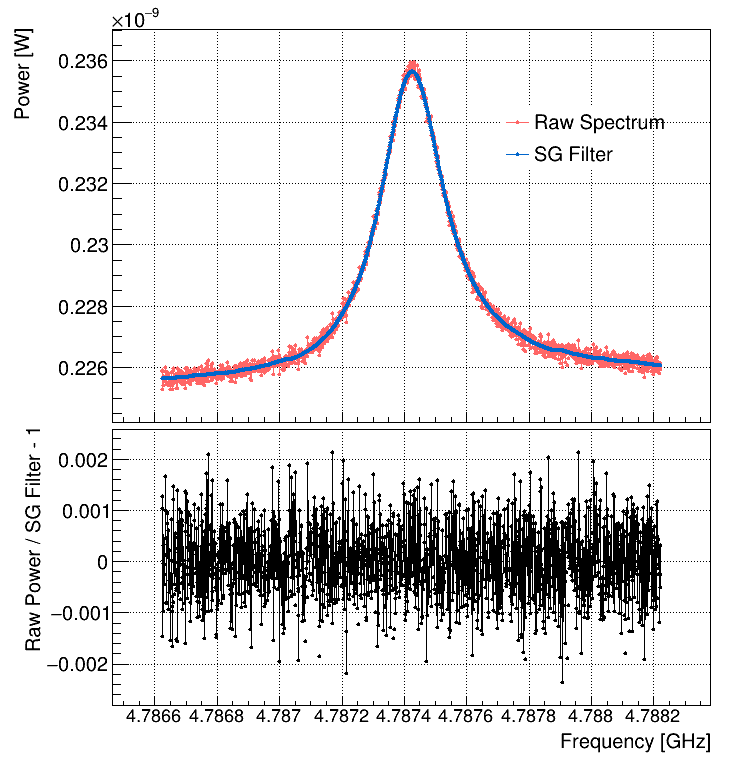
\includegraphics[width=8.6cm]{figures/RawPower_SGPower_Ratio_vs_Freq_Step_0100.png}
  \caption{Upper panel: The raw averaged power spectrum (red points) and the 
output of the SG filter (blue curve) of one scan. Lower panel: The normalized 
spectrum,  derived by taking the ratio of the raw spectrum to the SG filter 
and subtracting unity from the ratio. }
  \label{fig:raw_sg_power}
\end{figure}

\begin{figure} [htbp]
  \centering
  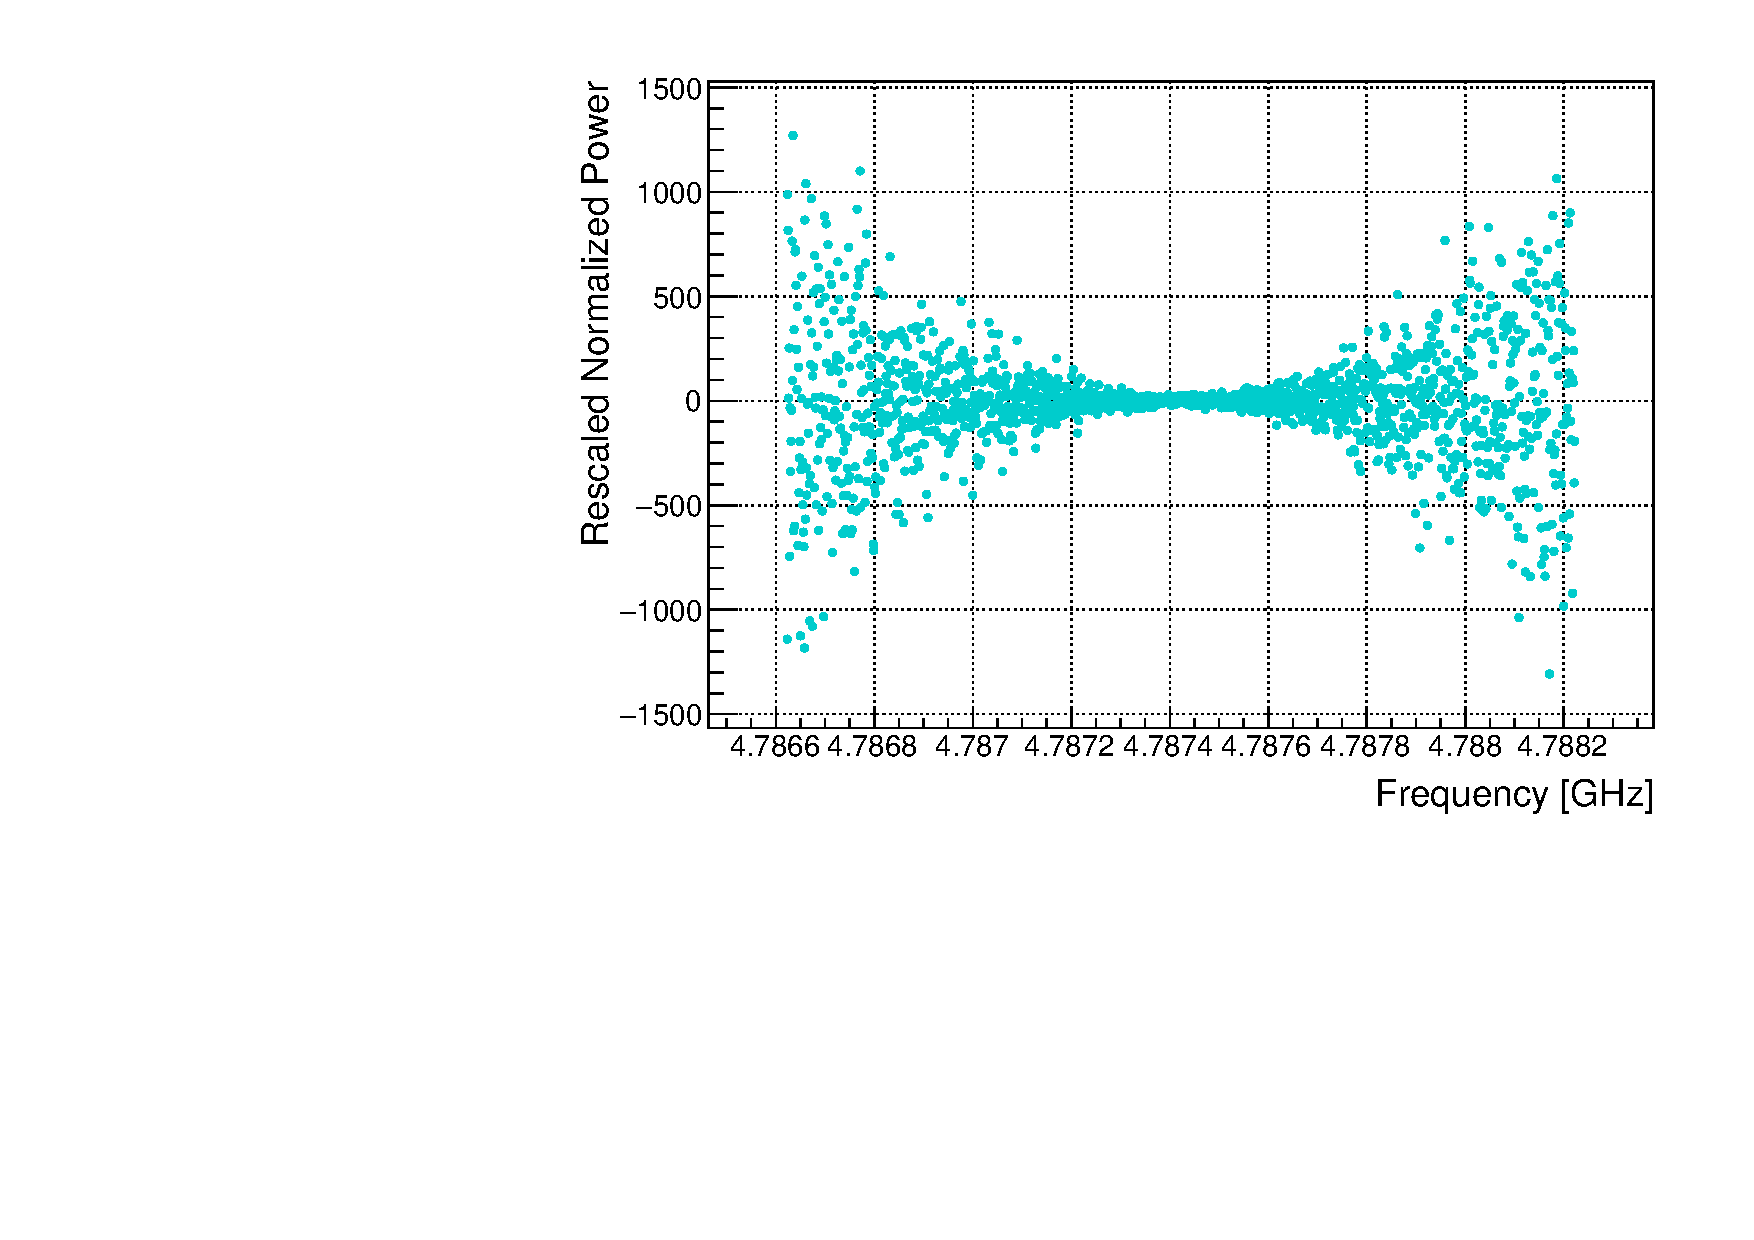
\includegraphics[width=8.6cm]{figures/RescaledPower_vs_Freq_Step_0100.pdf}
  \caption{
  The rescaled spectrum, obtained by multiplying the RDPs in the normalized 
spectrum with the ratio of the system noise power to the expected signal 
power of the KSVZ axion, 
with the Lorentzian response of the cavity taken into account.}
  \label{fig:rescaled_power}
\end{figure}



%First we will choose a window and a order, then move the window and fit the data a with a polynomial with chosen order, it is a kind of generalization  moving average characterized, if the windows is too big, then it will not remove small structures, if it too small, it may kill the signal, you can see that choosing an appropriate window is important, a way to test if the windows are appropriate is to see the system temperature calculated by  $\mu$ and $\sigma$.

%\begin{equation}
%    \label{eq:ts_mu}
%    \mu = k_{B} \cdot T_{S} \cdot \Delta f 
%\end{equation}
%\begin{equation}
%    \label{eq:ts_sigma}
%    \sigma = \frac{k_{B} \cdot T_{S} \cdot \Delta f}{\sqrt{N}}
%\end{equation}

%If we treat the spectrum after the SG filter as a pure noise, we know that the system temperature of a white noise can be calculated by $\mu$ and $\sigma$ (Eq.\eqref{eq:ts_mu}) (Eq.\eqref{eq:ts_sigma}),
%where $k_{B}$ is the Boltzmann constant, $T_{S}$ is the system temperature, $\Delta f$ is the frequency resolution and N is the number of averaging. \\
%If the chosen window is appropriate, the system temperature estimated from $\mu$ and $\sigma$ should be consistent  with each other. \\

%We also did some studies to check if the SG filter removed the axion signal. Assuming a signal bandwidth of 5 kHz, we added the signal into noise spectrum and applied the SG filter. The result shows that the filter does not suppress the axion signal as given in Fig.\ref{fig:weighted_snr}.

%about whether the sg filter will remove the Axion signal, assuming the Axion signal bandwidth is 5KHz, add the signal in a white noise and apply the sg filter , the results show that it will not affect much before and after use, after divide the sg filter result, we will subtract 1 to make the value become 1.

%\begin{figure}[h]
%    \begin{minipage}[h]{.5\textwidth}
%    \centering
%    \includegraphics[width=0.8\textwidth, height = 0.5\textwidth]{Figure/sg_simulation.png}
%    \caption{The simulation for testing the effect of SG filter.}
%    \label{fig:weighted_snr}
%%    \end{minipage}%
%\end{figure}
%\begin{figure}[h]
%    \begin{minipage}[t]{.5\textwidth}
%    \centering
%    \includegraphics[width=0.8\textwidth,height = 0.5\textwidth]{Figure/weighted_snr.png}
%    \caption{Weighed SNR}
%    \label{fig:weighted_snr}
%%    \end{minipage}%
%\end{figure}

\subsection{Combine the spectra with the weighting algorithm} 
\label{sec:weighting_algorithm}

The purpose of the weighting algorithm is to add the spectra from different 
resonant-frequency scans,
 particularly for the frequency bins that appear in multiple spectra.  
Each spectrum was collected with a different cavity resonant frequency. 
Therefore, if a signal appears in a certain frequency bin $j$, due to the
 difference in the resonant frequency and the Lorentzian response, the 
expected signal
 power will be different in each spectrum $i$. The weighting algorithm is 
expected to take this into account with a weight calculated for each bin $j$ of
 the rescaled spectrum $i$, as defined below: %in Eq.~\eqref{eq:weight}:
\begin{equation}
    \label{eq:weight}
    %    {w_{n}}^{i} = \frac{h \cdot p}{(\sigma_{n}^{i})^{2}}
    {w_{ijn}} = \frac{\Gamma_{ijn}}{(\sigma_{ij}^\text{res})^{2}}.
\end{equation}
Note, the symbol $\Gamma_{ijn}=1$ if the $j^\text{th}$ frequency bin in the 
$i^\text{th}$ rescaled spectrum correspond to the same frequency in 
the $n^\text{th}$ bin of the combined spectrum; otherwise, $\Gamma_{ijn}=0$.

The RDP $\delta^\text{com}_{n}$ and the standard deviation 
$\sigma^\text{com}_{n}$ of the $n^\text{th}$ bin in the combined spectrum are 
calculated using Eq.~\eqref{eq:comb_power} and Eq.~\eqref{eq:comb_sigma}, 
respectively. The SNR$^\text{com}_{n}$ is the ratio of 
$\delta^\text{com}_{n}$ to 
$\sigma^\text{com}_{n}$ as given in Eq.~\eqref{eq:comb_snr}. 
%Figure~\ref{fig:power_sigma_comb} and Fig.~\ref{fig:SNR_comb} show the power, 
%the standard deviation, and the SNR of the combined spectrum, respectively.
Figure~\ref{fig:power_sigma_comb} and Fig.~\ref{fig:SNR_comb} show the RDP, 
the standard deviation, and the SNR of the combined spectrum, respectively.

\begin{equation}
    \label{eq:comb_power}
%    \delta_{n}^\text{com} = \frac{ \sum_{1}^{k}\left(\delta_{ij}^\text{res} \cdot {w_{ij}}\right)}{\sum_{1}^{k} {w_{ij}}},
    \delta_{n}^\text{com} = \frac{ \sum\limits_{i}\sum\limits_{j}\left(\delta_{ij}^\text{res} \cdot {w_{ijn}}\right)}{\sum\limits_{i}\sum\limits_{j} {w_{ijn}}},
\end{equation}
\begin{equation}
    \label{eq:comb_sigma}
%    \sigma_{n}^\text{com} = \frac{ \sqrt{\sum_{1}^{k}(\sigma_{ij}^\text{res} \cdot {w_{ij}})^2}}{\sum_{1}^{k} {w_{ij}}},
    \sigma_{n}^\text{com} = \frac{ \sqrt{\sum\limits_{i}\sum\limits_{j}(\sigma_{ij}^\text{res} \cdot {w_{ijn}})^2}}{\sum\limits_{i}\sum\limits_{j} {w_{ijn}}},
\end{equation}
\begin{equation}
    \label{eq:comb_snr}
%    \text{SNR}_{n}^\text{com} = \frac{\delta^\text{com}_{n}}{\sigma^\text{com}_{n}}= \frac{\sum_{1}^{k}\left(\delta_{ij}^{res} \cdot {w_{ij}}\right)}{ \sqrt{\sum_{1}^{k}(\sigma_{ij}^{res} \cdot {w_{ij}})^2}},
    \text{SNR}_{n}^\text{com} = \frac{\delta^\text{com}_{n}}{\sigma^\text{com}_{n}}= \frac{\sum\limits_{i}\sum\limits_{j}\left(\delta_{ij}^{res} \cdot {w_{ijn}}\right)}{ \sqrt{\sum\limits_{i}\sum\limits_{j}(\sigma_{ij}^{res} \cdot {w_{ijn}})^2}}.
\end{equation} 
For each bin $n$ in the combined spectrum, there are $m_n$ non-vanishing contributions to the sums above. In 
general, the value of $m_n$ is XXXX. 


\begin{figure}[h]
    \centering
    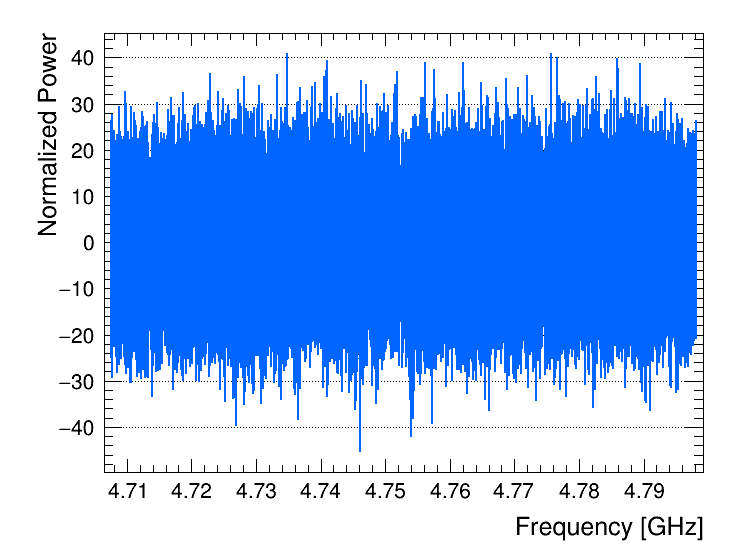
\includegraphics[width=8.6cm]{figures/Power_CombSpectrum_AxionRun_AllSteps_Rescan_SG4_W201_LqWeight.png}
    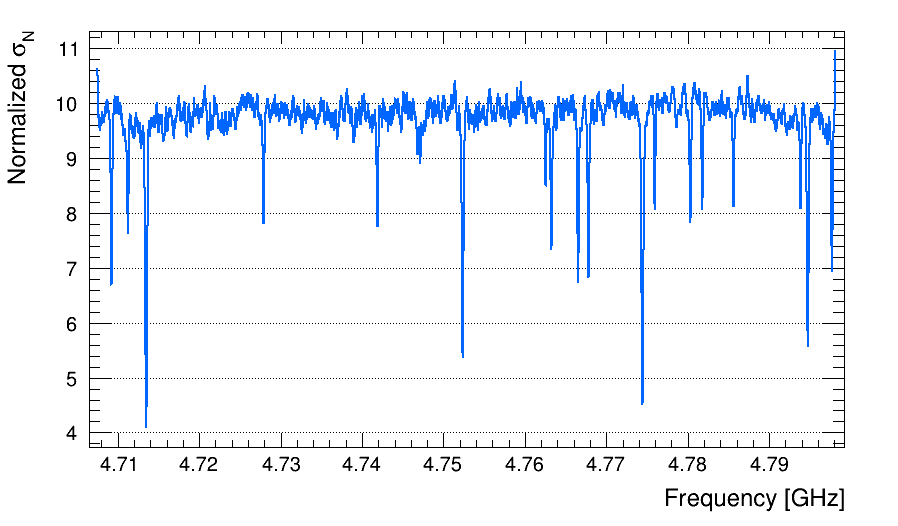
\includegraphics[width=8.6cm]{figures/Sigma_CombSpectrum_AxionRun_AllSteps_Rescan_SG4_W201_LqWeight.png}
    \caption{The combined RDP $\delta$ following Eq.~\eqref{eq:comb_power} 
(upper) and the standard deviation $\sigma$ derived from 
Eq.~\eqref{eq:comb_sigma} (lower).}
    \label{fig:power_sigma_comb}
\end{figure}

\begin{figure}[hbt!]
    \centering
    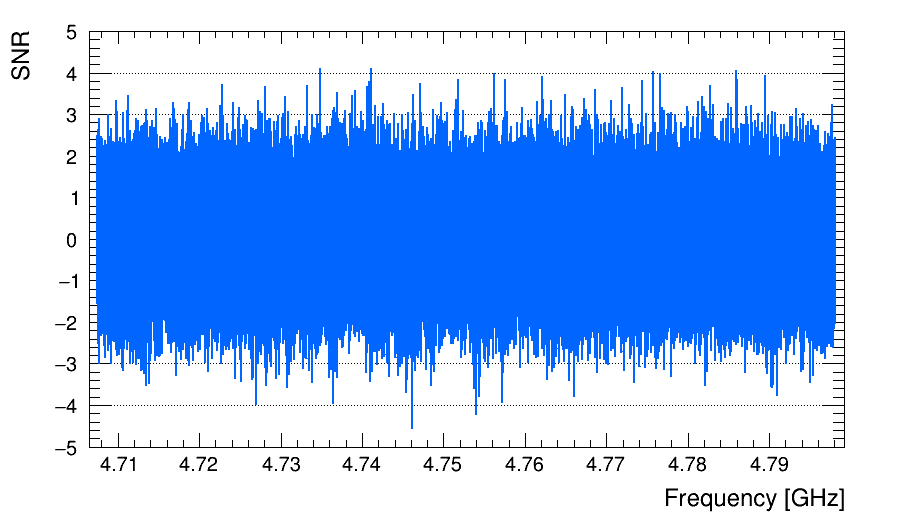
\includegraphics[width=8.6cm]{figures/SNR_CombSpectrum_AxionRun_AllSteps_Rescan_SG4_W201_LqWeight.png}
    \caption{The signal-to-noise ratio (SNR) calculated using 
Eq.\eqref{eq:comb_snr} of the combined spectrum. }
    \label{fig:SNR_comb}
\end{figure}


%where ${\delta_n^i}$ and ${\sigma_n^i}$ are the measured power and the corresponding standard deviation of the ${n^{\mathrm{th}}}$ frequency bin of the ${i^{\mathrm{th}}}$ spectrum., From the weighted power in ${n^{th}}$ bin in Eq.\eqref{eq:weighted_power}, and weighted $\sigma$ in Eq.\eqref{eq:weighted_sigma}, we can get our Signal to noise ratio as Eq.\eqref{eq:weighted_SNR}

\subsection{Merge bins}
\label{sec:merge}

The expected axion bandwidth is about 5~kHz at the frequency of $\approx5$~GHz. 
In this paper, the interested frequency range is \flo -- \fhi~GHz and the bin 
width is 1~kHz. Therefore, in order to maximize the SNR, a running window of 
five consecutive bins in the combined spectrum are merged to construct a 
final spectrum.
The purpose of using a running window is to avoid the signal power broken 
into different neighboring bins of the merged spectrum. 
%Before defining the 
%weights for merging, 
%the power and the standard deviation of each bin in the combined spectrum are 
%multiplied with $M=5$: $\delta^{c}_n \rightarrow M\delta^\text{com}_n$ and 
%$\sigma^{c}_n \rightarrow M \sigma^\text{com}_n$. This rescaling gives the 
%expected mean of the normalized power $\mu^\text{com}_k = 1$ if a KSVZ axion 
%signal power leaves a fraction 1/$M$ of its power in the $k^\text{th}$ 
%bin of the combined spectrum.
Then the maximum likelihood weights, defined in Eq.~\eqref{eq:merge_weight} 
based on the Maxwellian line shape for axions [Eq.~\eqref{eq:simplesignal}], 
are used to build the merged spectrum: 
\begin{equation}
    \label{eq:merge_weight}
    w_{gk} = \frac{L_{gk}}{(\sigma_{g+k-1}^\text{com})^{2}},
\end{equation}
 in which 
\begin{equation}
    \label{eq:Lq_integtal}
    L_{gk} = \int_{f_a +\delta f_m + (k-1)\Delta f_\text{bin}}^{f_a +\delta f_m + k\Delta f_\text{bin}} \mathcal{F}(f) \,df. 
\end{equation}
Here, $g = 1,..,N-M+1$ is the index for 
the frequency bins in the final spectrum and $M=5$ is the number of merged bins. 
The total number of bins in the combined (final merged) spectrum is
$N$ ($N-M+1$). 
The variable $k$ is the index within the group of bins for merging and 
$k = 1,..,M$. 
The frequency $f_a=\left.\ma c^2\middle/h\right.$ is 
the axion frequency, $\delta f_m$ is the misalignment between $f_a$ and the lower 
boundary of the $g^\text{th}$ bin 
in the combined spectrum. 
The function $\mathcal{F}(f)$ has been defined in Eq.~\eqref{eq:simplesignal}. 

%where $L_q$ is the integral of the line shape from the lower edge to higher 
%edge of ${q^{th}}$ bin. 
The RDP, the standard deviation, and the SNR of the merged spectrum are:

%We have a weight Eq.\eqref{eq:merge_weight}, where Lq is the area in ${q^{th}}$ bin and $\sigma_{q}$ is the weighted $\sigma$ in the $q^{\mathrm{th}}$ bin , Eq.\eqref{eq:axion_line_shape} is the axion CDM(cold dark matter) line shape, where $\big \langle \beta^{2} \big \rangle = \big \langle v^{2} \big \rangle /c^{2}$ and $\big \langle v^{2} \big \rangle = (270km/s)^{2}\ , \big \langle v^{2} \big \rangle$ is the squared virial velocity. Eq.\eqref{eq:L_q_integtal},

\begin{equation}
    \delta_{g}^\text{merged} = M \frac{ \sum\limits_{k = 1}^{M}\left(\delta_{g+k-1}^\text{com} \cdot {w_{gk}}\right)}{\sum\limits_{k = 1}^{M} {w_{gk}}},
    \label{eq:merged_power}
\end{equation}

\begin{equation}
    \sigma_{g}^\text{merged} =  M \frac{ \sqrt{\sum\limits_{k = 1}^{M} \left(\sigma_{g+k-1}^\text{com} \cdot {w_{gk}}\right)^2}}{\sum\limits_{k = 1}^{M} {w_{gk}}},
    \label{eq:merged_sigma}
\end{equation}

\begin{equation}
    \label{eq:merged_snr}
    \text{SNR}_{g}^\text{merged} = \frac{\delta^\text{merged}_{g}}{\sigma^\text{merged}_{g}} = \frac{\sum\limits_{k = 1}^{M}\left(\delta_{g+k-1}^\text{com} \cdot {w_{gk}}\right)}{ \sqrt{\sum\limits_{k = 1}^{M} \left(\sigma_{g+k-1}^\text{com} \cdot {w_{gk}}\right)^2}},
\end{equation}
%where $M=5$ is the number of merged bins. $g = 1,..,N-M+1$ is the index for 
%the frequency bins in the final spectrum.  
%The total number of bins in the combined (final merged) spectrum is 
%$N$ ($N-M+1$). 
Without the multiplication factor $M$ in 
Eqs.~\eqref{eq:merged_power}--~\eqref{eq:merged_sigma}, the results of the two equations 
simply provide the weighted averages of RDP and standard deviation, respectively.   
Assuming that the axion signal leaves a fraction $1/M$ of its power in one 
frequency bin, adding the factor $M$ converts the average into a summation of the values in the 
five bins and can recover the full size of the axion signal. 

%Adding adjacent bin with a weight Eq.\eqref{eq:merged_power} Eq.\eqref{eq:merged_sigma}, where k is the number of adjacent bin to be merged, q is ${q^{th}}$ merged bin, with Eq.\eqref{eq:merged_sigma}, we can get our weighted merged power spectrum FIG.\ref{fig:merged_data}.


\subsection{Rescan and set limits on \gagg} 
Before the collection of the CD102 data, a 5$\sigma$ SNR target was chosen, 
which corresponds to a candidate threshold of 3.355$\sigma$ at 95\% confidence.
 After the merging as described in Sec.~\ref{sec:merge}, if there were 
any potential signal with an SNR larger than 
3.355, a rescan would be proceeded to check if it were a real signal 
or a statistical fluctuation. 
The procedure of the CD102 data taking was to perform a rescan after 
covering every 10~MHz; the rescan was done by adjusting the tuning rod of the 
cavity so to match the resonant frequency to the frequency of the candidate. 
In total, 22 candidates with an SNR greater than 3.355 were found. 
Among them, 17 candidates were from the fluctuations because they were gone 
after a few rescans. 
The remaining five candidates, in the frequency ranges of 
4.710170 -- 4.710190~GHz and 4.747301 -- 4.747380~GHz, reached an SNR greater than 
4 after rescanning. The signals in the second frequency 
range were detected via a portable antenna outside the DR and found 
to come from the instruments in the laboratory, while the signals 
in the first frequency range were weaker but still present after 
turning off the external magnetic field. 
Therefore, these five candidates are considered external signals and 
no limits are placed for the above two frequency ranges.  
More details can be found in the 
TASEH instrumentation paper~\cite{TASEHInstrumentation}. 
Figure~\ref{fig:power_sigma_merged} and Fig.~\ref{fig:SNR_merged} show the 
RDP, the standard deviation, and the SNR of the merged spectrum after 
including data from both the original scans and the rescans, respectively. 

Since no candidates were found after the rescan, an upper limit on 
the signal power $P_s$ is derived by setting $P_s$ equal to 
$5\sigma_{g}^\text{merged}$ for a certain frequency bin $g$ in the merged 
spectrum.  Then, the 95\% C.L. limits on the dimensionless parameter 
\ggamma\ and the axion-two-photon coupling \gagg\ could be derived 
according to Eq.~\eqref{eq:ps} and Eq.~\eqref{eq:grelation}. 
See Sec.~\ref{sec:results} for the final limits including the systematic 
uncertainties.

\begin{figure}[h]
    \centering
    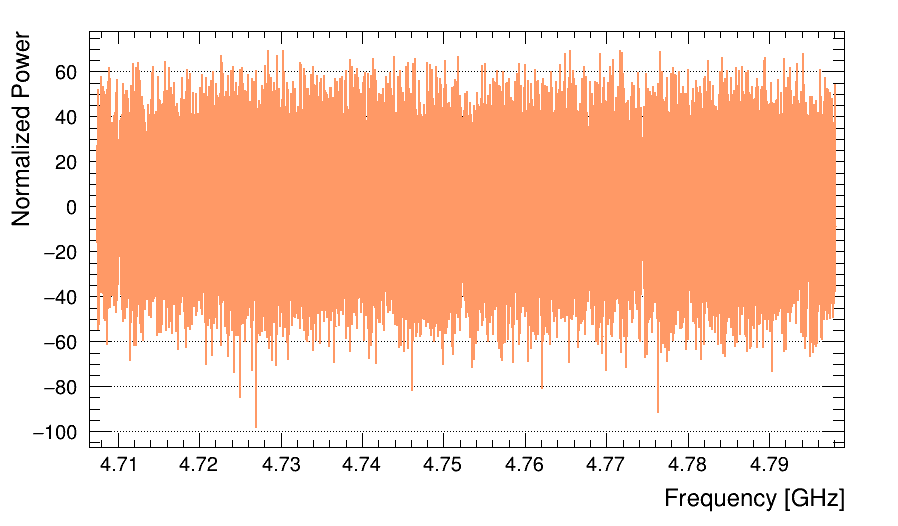
\includegraphics[width=8.6cm]{figures/Power_GrandSpectrum_AxionRun_AllSteps_Rescan_Merged_5bin_SG4_W201_LqWeight.png}
    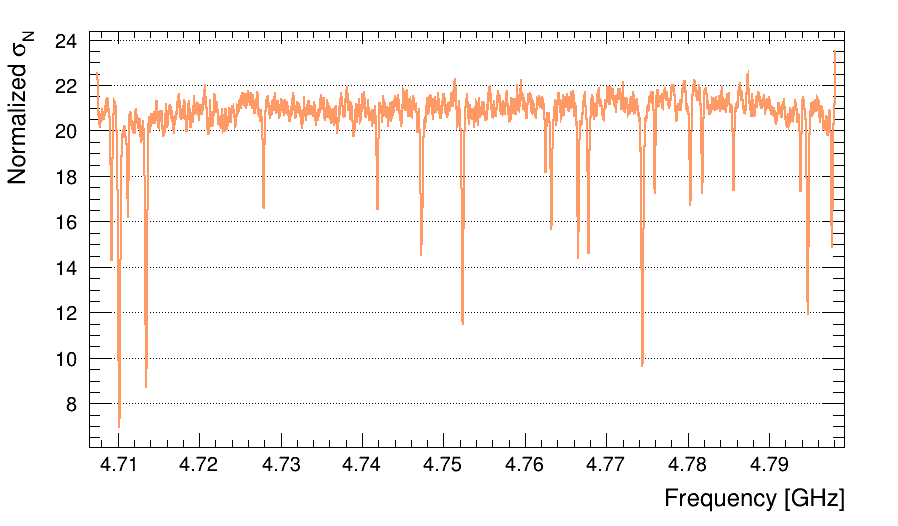
\includegraphics[width=8.6cm]{figures/Sigma_GrandSpectrum_AxionRun_AllSteps_Rescan_Merged_5bin_SG4_W201_LqWeight.png}
    \caption{The merged RDP $\delta$ following Eq.~\eqref{eq:merged_power} 
(upper) and the standard deviation $\sigma$ derived from Eq.~\eqref{eq:merged_sigma} (lower). The results shown were obtained using data from both the 
original scans and the rescans.}
    \label{fig:power_sigma_merged}
\end{figure}

\begin{figure}[hbt!]
    \centering
    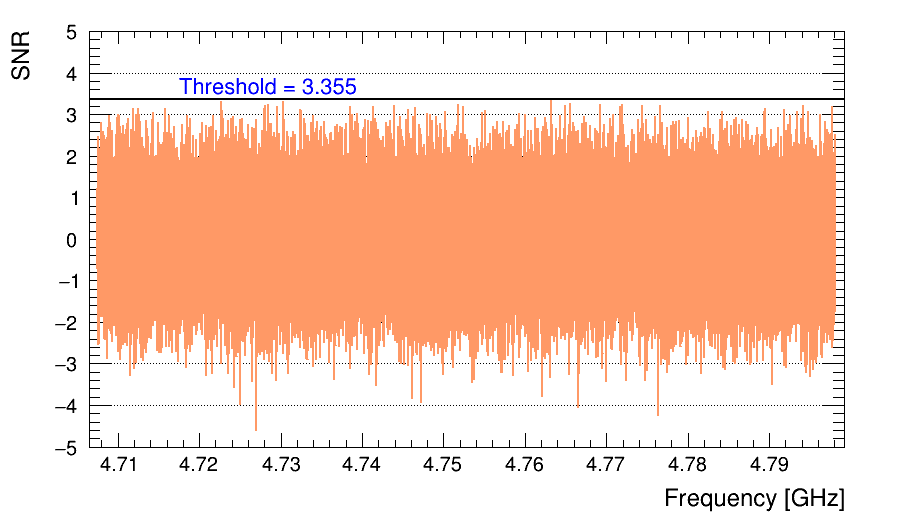
\includegraphics[width=8.6cm]{figures/SNR_GrandSpectrum_AxionRun_AllSteps_Rescan_Merged_5bin_SG4_W201_LqWeight.png}
    \caption{The signal-to-noise ratio (SNR) calculated using Eq.~\eqref{eq:merged_snr} for the merged spectrum including data from both the original 
scans and the rescans. No candidate exceeds the threshold of 
$3.355\sigma$ (solid-black horizontal line). }
    \label{fig:SNR_merged}
\end{figure}
